\documentclass[a4paper,12pt]{article}

\usepackage[utf8x]{inputenc}
\usepackage[T2A]{fontenc}
\usepackage[english, russian]{babel}

% Опционно, требует  apt-get install scalable-cyrfonts.*
% и удаления одной строчки в cyrtimes.sty
% Сточку не удалять!
% \usepackage{cyrtimes}

% Картнки и tikz
\usepackage{graphicx}
\usepackage{tikz}
\usetikzlibrary{snakes,arrows,shapes}


% Некоторая русификация.
\usepackage{misccorr}
\usepackage{indentfirst}
\renewcommand{\labelitemi}{\normalfont\bfseries{--}}

% Увы, поля придётся уменьшить из-за листингов.
\topmargin -1cm
\oddsidemargin -0.5cm
\evensidemargin -0.5cm
\textwidth 17cm
\textheight 24cm

\sloppy

% Оглавление в PDF
\usepackage[
bookmarks=true,
colorlinks=true, linkcolor=black, anchorcolor=black, citecolor=black, menucolor=black,filecolor=black, urlcolor=black,
unicode=true
]{hyperref}

% Для исходного кода в тексте
\newcommand{\Code}[1]{\texttt{#1}}

\usepackage{verbatim}
\usepackage{fancyvrb}
\fvset{frame=leftline, fontsize=\small, framerule=0.4mm, rulecolor=\color{darkgray}, commandchars=\\\{\}}
\renewcommand{\theFancyVerbLine}{\small\arabic{FancyVerbLine}}


\title{Отчёт по лабораторной работе \\ <<Динамическая IP-маршрутизация>> \\ Вариант №6}
\author{(Овчинников Владислав Александрович)}

\begin{document}

\maketitle

\tableofcontents

\section{Настройка сети}

\subsection{Топология сети}

Топология сети и используемые IP-адреса показаны на рисунке~\ref{fig:network}.

\begin{figure}
\centering
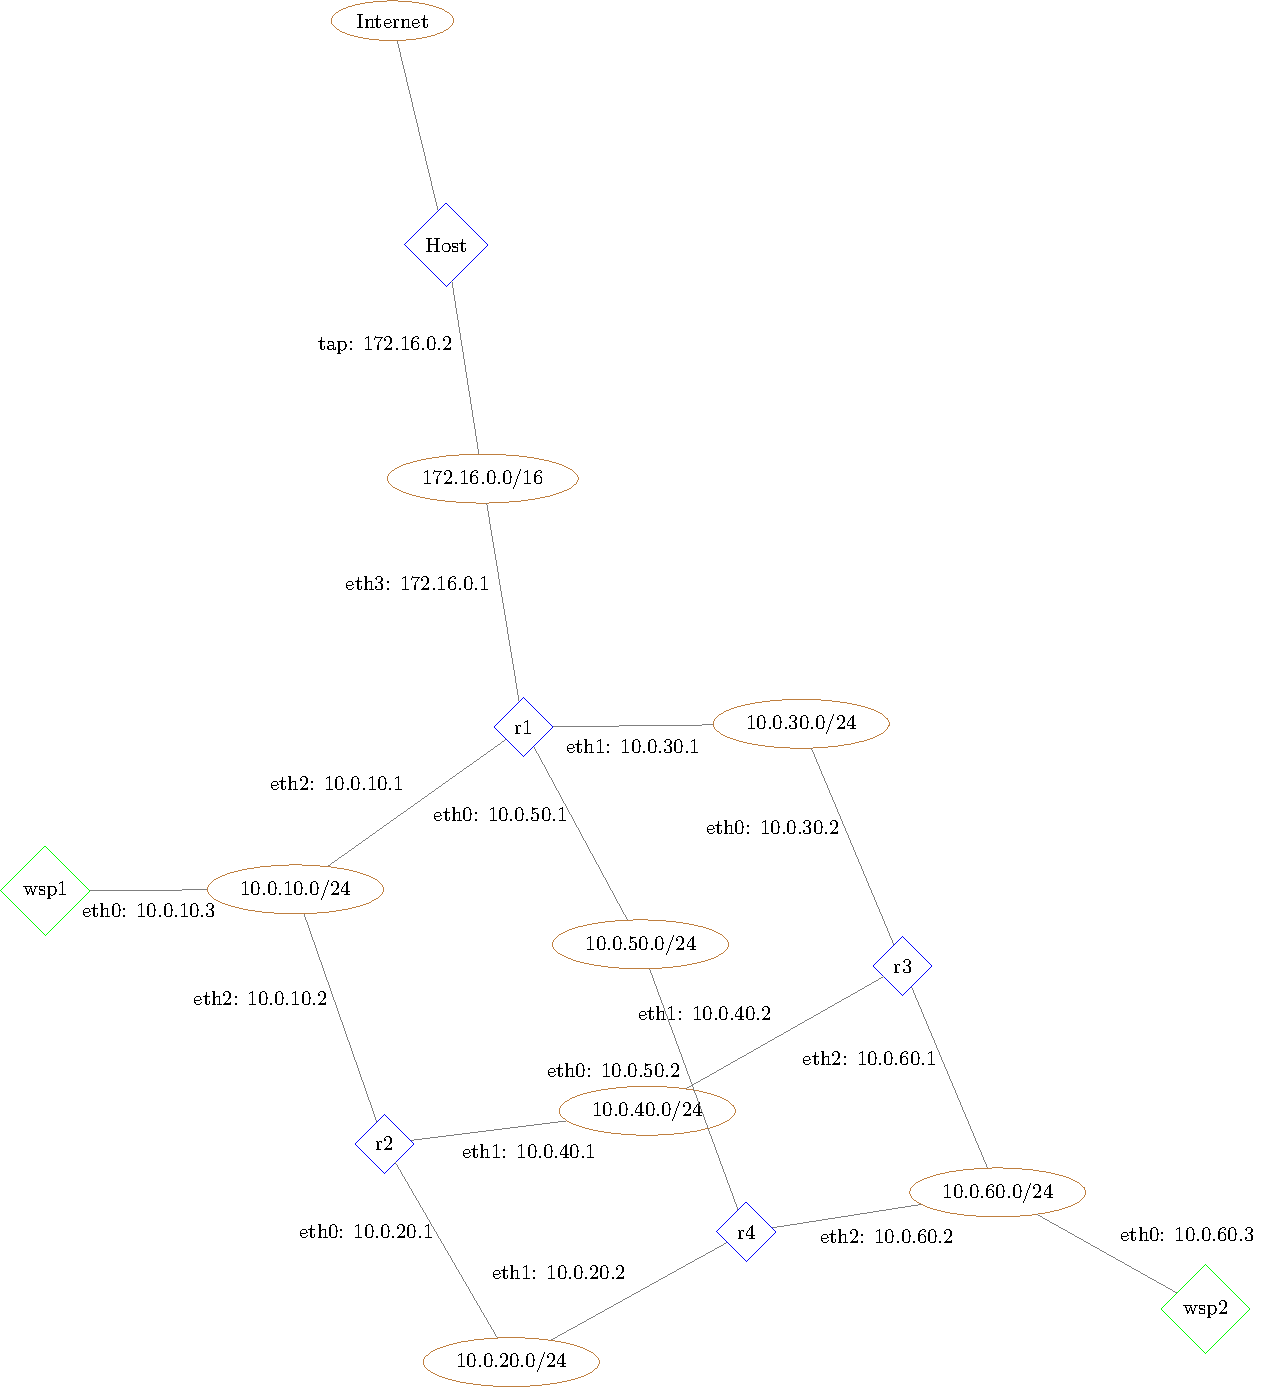
\includegraphics[width=0.8\textwidth]{includes/network_gv.pdf}
\caption{Топология сети}
\label{fig:network}
\end{figure}

Динамическая маршрутизация используется на всех узлах сети, так как все узлы подключены к сегментам сети, к которым подключены более чем один маршрутизатор. Таким образом, перечень узлов, на которых используется динамическая IP-маршрутизация: r1, r2, r3, r4, wsp1, wsp2.

\newpage

\subsection{Назначение IP-адресов}

Для настройки сiiетевых интерфейсов и присвоения им соответствующего IP-адреса были изменен файл /etc/network/interfaces соответствующих узлов.

Ниже приведён файл сетевой настройки маршрутизатора \textbf{r1}:

\begin{Verbatim}
auto lo
iface lo inet loopback

auto eth0
iface eth0 inet static
address 10.0.50.1
netmask 255.255.255.0

auto eth1
iface eth1 inet static
address 10.0.30.1
netmask 255.255.255.0

auto eth2
iface eth2 inet static
address 10.0.10.1
netmask 255.255.255.0
\end{Verbatim}

Ниже приведён файл сетевой настройки маршрутизатора \textbf{r2}:

\begin{Verbatim}
auto lo
iface lo inet loopback

auto eth0
iface eth0 inet static
address 10.0.20.1
netmask 255.255.255.0

auto eth1
iface eth1 inet static
address 10.0.40.1
netmask 255.255.255.0

auto eth2
iface eth2 inet static
address 10.0.10.2
netmask 255.255.255.0
\end{Verbatim}

Ниже приведён файл сетевой настройки маршрутизатора \textbf{r3}:

\begin{Verbatim}
auto lo
iface lo inet loopback

auto eth0
iface eth0 inet static
address 10.0.30.2
netmask 255.255.255.0

auto eth1
iface eth1 inet static
address 10.0.40.2
netmask 255.255.255.0

auto eth2
iface eth2 inet static
address 10.0.60.1
netmask 255.255.255.0
\end{Verbatim}

Ниже приведён файл сетевой настройки маршрутизатора \textbf{r4}:

\begin{Verbatim}
auto lo
iface lo inet loopback

auto eth0
iface eth0 inet static
address 10.0.50.2
netmask 255.255.255.0

auto eth1
iface eth1 inet static
address 10.0.20.2
netmask 255.255.255.0

auto eth2
iface eth2 inet static
address 10.0.60.2
netmask 255.255.255.0
\end{Verbatim}

Ниже приведён файл сетевой настройки рабочей станции \textbf{wsp1}.

\begin{Verbatim}
auto lo
iface lo inet loopback

auto eth0
iface eth0 inet static
address 10.0.10.3
netmask 255.255.255.0
gateway 10.0.10.1
\end{Verbatim}

Ниже приведён файл сетевой настройки рабочей станции \textbf{wsp2}.

\begin{Verbatim}
auto lo
iface lo inet loopback

auto eth0
iface eth0 inet static
address 10.0.60.3
netmask 255.255.255.0
gateway 10.0.60.1
\end{Verbatim}


\subsection{Настройка протокола RIP}

\textbf{Quagga} - пакет свободного программного обеспечения, поддерживающий протоколы динамической маршрутизации IP. Компьютер с установленным и сконфигурированным пакетом Quagga способен поддерживать множество протоколов динамической маршрутизации, одним из которых является \textbf{Routing Information Protocol (RIP)}.

\textbf{Протокол маршрутной информации} (Routing Information Protocol - RIP) - один из самых простых протоколов маршрутизации. Применяется в небольших компьютерных сетях, позволяет маршрутизаторам динамически обновлять маршрутную информацию (направление и дальность в хопах), получая ее от соседних маршрутизаторов.

RIP - протокол дистанционно-векторной маршрутизации, который оперирует транзитными участками (хоп) в качестве метрики маршрутизации. Максимальное количество транзитных участков, разрешенное в RIP - 15 (метрика 16 означает "бесконечно большую метрику"). Каждый RIP-маршрутизатор по умолчанию вещает в сеть свою полную таблицу маршрутизации раз в 30 секунд, довольно сильно нагружая низкоскоростные линии связи. В современных сетевых средах RIP - не самое лучшее решение для выбора в качестве протокола маршрутизации, так как его возможности уступают более современным протоколам, таким как EIGRP, OSPF. Ограничение на 15 транзитных участков не дает применять его в больших сетях. Преимущество этого протокола - простота конфигурирования.

Так как в данной сети четыре маршрутизатора и две рабочии станции, которые связаны с несколькими маршрутизаторами, требовалось сконфигурировать RIP на всех узлах сети.

Ниже приведен файл \Code{/etc/quagga/ripd.conf} маршрутизатора \textbf{r1}:

\begin{Verbatim}
router rip

network eth0
network eth1
network eth2

timers basic 10 60 120

redistribute kernel

log file /var/log/quagga/ripd.log
\end{Verbatim}

Ниже приведен файл \Code{/etc/quagga/ripd.conf} маршрутизатора \textbf{r2}:

\begin{Verbatim}
router rip

network eth0
network eth1
network eth2

timers basic 10 60 120

redistribute kernel
redistribute connected

log file /var/log/quagga/ripd.log
\end{Verbatim}

Ниже приведен файл \Code{/etc/quagga/ripd.conf} маршрутизатора \textbf{r3}:

\begin{Verbatim}
router rip

network eth0
network eth1
network eth2

timers basic 10 60 120

redistribute kernel
redistribute connected

log file /var/log/quagga/ripd.log
\end{Verbatim}

Ниже приведен файл \Code{/etc/quagga/ripd.conf} маршрутизатора \textbf{r4}:

\begin{Verbatim}
router rip

network eth0
network eth1
network eth2

timers basic 10 60 120

redistribute kernel
redistribute connected

log file /var/log/quagga/ripd.log
\end{Verbatim}

Ниже приведен файл \Code{/etc/quagga/ripd.conf} рабочей станции \textbf{wsp1}, связанной с несколькими маршрутизаторам:

\begin{Verbatim}
router rip

network eth0

timers basic 10 60 120

redistribute kernel
redistribute connected

log file /var/log/quagga/ripd.log
\end{Verbatim}

Ниже приведен файл \Code{/etc/quagga/ripd.conf} рабочей станции \textbf{wsp2}, связанной с несколькими маршрутизаторам:

\begin{Verbatim}
router rip

network eth0

timers basic 10 60 120

redistribute kernel
redistribute connected

log file /var/log/quagga/ripd.log
\end{Verbatim}


\section{Проверка настройки протокола RIP}

Требовалось проверить правильность конфигурации RIP. Для этого был произведен вывод пути с помощью \textbf{traceroute}.

Вывод \textbf{traceroute} от узла \textbf{wsp1} до узла \textbf{wsp2} при нормальной работе сети:

\begin{Verbatim}
traceroute to 10.0.60.3 (10.0.60.3), 64 hops max, 40 byte packets
 1  10.0.10.2 (10.0.10.2)  8 ms  0 ms  0 ms
 2  10.0.30.2 (10.0.30.2)  31 ms  1 ms  0 ms
 3  10.0.60.3 (10.0.60.3)  11 ms  1 ms  1 ms
\end{Verbatim}

Вывод \textbf{traceroute} от узла \textbf{r1} до внешнего IP \textbf{5.255.255.77}:

\begin{Verbatim}
traceroute to 5.255.255.77 (5.255.255.77), 64 hops max, 40 byte packets
 1  172.16.0.1 (172.16.0.1)  0 ms  0 ms  0 ms
 2  192.168.0.1 (192.168.0.1)  3 ms  1 ms  1 ms
 3  90.154.77.227 (90.154.77.227)  2 ms  2 ms  2 ms
 4  77.37.250.200 (77.37.250.200)  2 ms  2 ms  2 ms
 5  87.226.221.170 (87.226.221.170)  12 ms  3 ms  3 ms
 6  213.59.212.217 (213.59.212.217)  2 ms 213.59.211.237 (213.59.211.237)  2 ms 188.254.25.77 (188.254.25.77)  2 ms
 7  * * *
 8  5.143.250.94 (5.143.250.94)  4 ms  3 ms  3 ms
 9  * * *
10  5.255.255.77 (5.255.255.77)  7 ms (TOS=96!)  6 ms  5 ms
\end{Verbatim}

Также для проверки RIP были перехвачены датаграммы UDP с помощью \textbf{tcpdump}.

Вывод сообщения RIP, перехваченного на маршрутизаторе \textbf{r4}:

\begin{Verbatim}
RIPv2, Response, length: 124, routes: 6
	  AFI: IPv4:         0.0.0.0/0 , tag 0x0000, metric: 2, next-hop: self
	  AFI: IPv4:       10.0.10.0/24, tag 0x0000, metric: 2, next-hop: self
	  AFI: IPv4:       10.0.20.0/24, tag 0x0000, metric: 2, next-hop: self
	  AFI: IPv4:       10.0.30.0/24, tag 0x0000, metric: 1, next-hop: self
	  AFI: IPv4:       10.0.40.0/24, tag 0x0000, metric: 1, next-hop: self
	  AFI: IPv4:       10.0.50.0/24, tag 0x0000, metric: 2, next-hop: self
\end{Verbatim}

Вывод таблицы RIP на маршрутизаторе \textbf{r4}:

\begin{Verbatim}
     Network            Next Hop         Metric From            Tag Time
R(n) 0.0.0.0/0          10.0.50.1             2 10.0.50.1         0 00:56
R(n) 10.0.10.0/24       10.0.20.1             2 10.0.20.1         0 01:00
C(i) 10.0.20.0/24       0.0.0.0               1 self              0
R(n) 10.0.30.0/24       10.0.60.1             2 10.0.60.1         0 00:54
R(n) 10.0.40.0/24       10.0.20.1             2 10.0.20.1         0 01:00
C(i) 10.0.50.0/24       0.0.0.0               1 self              0
C(i) 10.0.60.0/24       0.0.0.0               1 self              0
\end{Verbatim}

Вывод таблицы маршрутизации на маршрутизаторе \textbf{r4}:

\begin{Verbatim}
10.0.20.0/24 dev eth1  proto kernel  scope link  src 10.0.20.2 
10.0.50.0/24 dev eth0  proto kernel  scope link  src 10.0.50.2 
10.0.60.0/24 dev eth2  proto kernel  scope link  src 10.0.60.2 
10.0.30.0/24 via 10.0.60.1 dev eth2  proto zebra  metric 2 
10.0.40.0/24 via 10.0.20.1 dev eth1  proto zebra  metric 2 
10.0.10.0/24 via 10.0.20.1 dev eth1  proto zebra  metric 2 
default via 10.0.50.1 dev eth0  proto zebra  metric 2 
\end{Verbatim}

\section{Расщепленный горизонт и испорченные обратные обновления}

Опыты с расщепленным горизонтом и испорченными обратными обновлениями проводились на маршрутизаторе \textbf{r4}.

Вывод сообщений на маршрутизаторе \textbf{r4} с включенным расщепленным горизонтом и с включенными испорченными обновлениями:

\begin{Verbatim}
RIPv2, Response, length: 144, routes: 7
	  AFI: IPv4:         0.0.0.0/0 , tag 0x0000, metric: 2, next-hop: self
	  AFI: IPv4:       10.0.10.0/24, tag 0x0000, metric: 16, next-hop: 10.0.20.1
	  AFI: IPv4:       10.0.20.0/24, tag 0x0000, metric: 16, next-hop: self
	  AFI: IPv4:       10.0.30.0/24, tag 0x0000, metric: 2, next-hop: self
	  AFI: IPv4:       10.0.40.0/24, tag 0x0000, metric: 16, next-hop: 10.0.20.1
	  AFI: IPv4:       10.0.50.0/24, tag 0x0000, metric: 1, next-hop: self
	  AFI: IPv4:       10.0.60.0/24, tag 0x0000, metric: 1, next-hop: self
\end{Verbatim}

Вывод сообщений на маршрутизаторе \textbf{r4} с выключенным расщепленным горизонтом и c включенными испорченными обновлениями:

\begin{Verbatim}
RIPv2, Response, length: 144, routes: 7
	  AFI: IPv4:         0.0.0.0/0 , tag 0x0000, metric: 2, next-hop: self
	  AFI: IPv4:       10.0.10.0/24, tag 0x0000, metric: 2, next-hop: self
	  AFI: IPv4:       10.0.20.0/24, tag 0x0000, metric: 1, next-hop: self
	  AFI: IPv4:       10.0.30.0/24, tag 0x0000, metric: 2, next-hop: self
	  AFI: IPv4:       10.0.40.0/24, tag 0x0000, metric: 2, next-hop: 10.0.20.1
	  AFI: IPv4:       10.0.50.0/24, tag 0x0000, metric: 1, next-hop: self
	  AFI: IPv4:       10.0.60.0/24, tag 0x0000, metric: 1, next-hop: self
\end{Verbatim}

Объяснить разницу.

\section{Имитация устранимой поломки в сети}

Для имитации устранимой поломки в сети был отключен маршрутизатор \textbf{r3}.

Вывод с помощью \textbf{traceroute} пути от узла \textbf{wsp1} до узла \textbf{wsp2} до отключения маршрутизатора \textbf{r3}:

\begin{Verbatim}
traceroute to 10.0.60.3 (10.0.60.3), 64 hops max, 40 byte packets
 1  10.0.10.2 (10.0.10.2)  0 ms  0 ms  0 ms
 2  10.0.40.2 (10.0.40.2)  0 ms  0 ms  0 ms
 3  10.0.60.3 (10.0.60.3)  0 ms  0 ms  0 ms
\end{Verbatim}

Вывод таблицы RIP непосредственно перед истечением таймера устаревания (на маршрутизаторе-соседе отключенного \textbf{r2}):

\begin{Verbatim}
     Network            Next Hop         Metric From            Tag Time
R(n) 0.0.0.0/0          10.0.10.1             2 10.0.10.1         0 00:59
C(i) 10.0.10.0/24       0.0.0.0               1 self              0
C(i) 10.0.20.0/24       0.0.0.0               1 self              0
R(n) 10.0.30.0/24       10.0.40.2             2 10.0.40.2         0 00:02
C(i) 10.0.40.0/24       0.0.0.0               1 self              0
R(n) 10.0.50.0/24       10.0.10.1             2 10.0.10.1         0 00:59
R(n) 10.0.60.0/24       10.0.40.2             2 10.0.40.2         0 00:02
\end{Verbatim}

Перестроенная таблица на маршрутизаторе \textbf{r3}

\begin{Verbatim}
     Network            Next Hop         Metric From            Tag Time
R(n) 0.0.0.0/0          10.0.10.1             2 10.0.10.1         0 00:49
C(i) 10.0.10.0/24       0.0.0.0               1 self              0
C(i) 10.0.20.0/24       0.0.0.0               1 self              0
R(n) 10.0.30.0/24       10.0.10.1             2 10.0.10.1         0 00:49
C(i) 10.0.40.0/24       0.0.0.0               1 self              0
R(n) 10.0.50.0/24       10.0.10.1             2 10.0.10.1         0 00:49
R(n) 10.0.60.0/24       10.0.20.2             2 10.0.20.2         0 00:57
\end{Verbatim}

Вывод с помощью \textbf{traceroute} от узла \textbf{wsp1} до узла \textbf{wsp2} после того, как служба RIP перестроила таблицы маршрутизации.

\begin{Verbatim}
traceroute to 10.0.60.3 (10.0.60.3), 64 hops max, 40 byte packets
 1  10.0.10.1 (10.0.10.1)  10 ms  0 ms  0 ms
 2  10.0.50.2 (10.0.50.2)  11 ms  0 ms  0 ms
 3  10.0.60.3 (10.0.60.3)  9 ms  0 ms  1 ms
\end{Verbatim}

\section{Имитация неустранимой поломки в сети}

Для имитации неустранимой поломки в сети был отключен маршрутизатор \textbf{r4}, что привело к недостижимости узла \textbf{wsp2}.

RIP-таблица на маршрутизаторе \textbf{r2} до отключения маршрутизатора \textbf{r4}:

\begin{Verbatim}
     Network            Next Hop         Metric From            Tag Time
R(n) 0.0.0.0/0          10.0.10.1             2 10.0.10.1         0 00:54
C(i) 10.0.10.0/24       0.0.0.0               1 self              0
C(i) 10.0.20.0/24       0.0.0.0               1 self              0
R(n) 10.0.30.0/24       10.0.10.1             2 10.0.10.1         0 00:54
C(i) 10.0.40.0/24       0.0.0.0               1 self              0
R(n) 10.0.50.0/24       10.0.10.1             2 10.0.10.1         0 00:54
R(n) 10.0.60.0/24       10.0.20.2             2 10.0.20.2         0 00:52
\end{Verbatim}

Перестроенная RIP-таблица на маршрутизаторе \textbf{r2} после отключения маршрутизатора \textbf{r4}, где видна 16-ая метрика:

\begin{Verbatim}
     Network            Next Hop         Metric From            Tag Time
R(n) 0.0.0.0/0          10.0.10.1             2 10.0.10.1         0 00:53
C(i) 10.0.10.0/24       0.0.0.0               1 self              0
C(i) 10.0.20.0/24       0.0.0.0               1 self              0
R(n) 10.0.30.0/24       10.0.10.1             2 10.0.10.1         0 00:53
C(i) 10.0.40.0/24       0.0.0.0               1 self              0
R(n) 10.0.50.0/24       10.0.10.1             2 10.0.10.1         0 00:53
R(n) 10.0.60.0/24       10.0.20.2            16 10.0.20.2         0 01:58
\end{Verbatim}

Перестроенная RIP-таблица на рабочей станции \textbf{wsp1} после отключения маршрутизатора \textbf{wsp1}, где видна 16-ая метрика:

\begin{Verbatim}
     Network            Next Hop         Metric From            Tag Time
R(n) 0.0.0.0/0          10.0.10.1             2 10.0.10.1         0 00:57
C(i) 10.0.10.0/24       0.0.0.0               1 self              0
R(n) 10.0.20.0/24       10.0.10.2             2 10.0.10.2         0 00:53
R(n) 10.0.30.0/24       10.0.10.1             2 10.0.10.1         0 00:57
R(n) 10.0.40.0/24       10.0.10.2             2 10.0.10.2         0 00:53
R(n) 10.0.50.0/24       10.0.10.1             2 10.0.10.1         0 00:57
R(n) 10.0.60.0/24       10.0.10.1            16 10.0.10.1         0 01:29
\end{Verbatim}

Сообщение протокола RIP с 16-ой метрикой, перехваченное на рабочей станции \textbf{wsp1}:

\begin{Verbatim}
RIPv2, Response, length: 84, routes: 4
  AFI: IPv4:         0.0.0.0/0 , tag 0x0000, metric: 1, next-hop: self
  AFI: IPv4:       10.0.30.0/24, tag 0x0000, metric: 1, next-hop: self
  AFI: IPv4:       10.0.50.0/24, tag 0x0000, metric: 1, next-hop: self
  AFI: IPv4:       10.0.60.0/24, tag 0x0000, metric: 16, next-hop: self
\end{Verbatim}

\section{Выводы}

В процессе выполнения данной лабораторной работы были выполнены следующие поставленные задачи:

1. Построена и сконфигурирована сеть в соответствии с поставленным вариантом.

2. Настроены сетевые интерфейсы у виртуальных машин.

3. Сконфигурирован протокол RIP с помощью ПО Quagga и конфигурационного файла /etc/quagga/ripd.conf.

4. Настроен подключения к внешней сети из виртуальных машин и выход в Интернет.

5. Протестирован и проверена настройка динамической маршрутизации и автоматическое заполнение маршрутных таблиц.

6. Проведены опыты с расщепленным горизонтом и испорченным обратным маршрутом.

7. Проведен опыт с устранением поломки в сети (при перестроении маршрута).

8. Проведен опыт, когда невозможно устранить поломку в сети и узел полностью недостижим.

Таким образом, все поставленные задачи были выполнены.

\end{document}
